\section{Protocol}
\label{sec:protocol}
To provide some context for the envirionment in which the proposed protocol interacts, we give some assumptions describing the status quo.

\subsection{Assumptions}
\subsubsection{Ethical Hacker - perspective}
\begin{enumerate}
	\item We assume it is not always as easy and/or attractive for whitehat hackers/ethical hackers to publish an exploit and retrieve an accompanying financial reward for the publication. This assumption is based on popular media such as darknet diaries, posts on news.ycombinator.com, hackernoon and possibly other sources. This assumption is based on (a combination of) the following sub-assumptions:
	\begin{enumerate}
		\item Vulnerabilities may be discovered at small/non-profit software development companies that have not allocated a large budget fraction to security.
		\item Ambiguity in the specification of the bug bounty/reward program may be interpreted in the advantage of the company during triage.
		\item The triage process may take a relatively long time, requiring the ethical hacker to have sufficient funds to sustain living costs coverage untill the pay-out.
		\item A conservative/carefullness in the ethical hacker towards approaching the company with respect to the legality of discovering the vulnerability may hinder/slow down the vulnerability disclosure process.
		\item The effort required contact the company and convince them of the seriousness of the bug may consume unnecessary resources.
	\end{enumerate}
\end{enumerate}

\subsubsection{Company - perspective}
\begin{enumerate}
	\item We assume cyber security vulnerabilities become increasingly more relevant in our increasingly more digitized world. This assumption may be seen as being substantiated by for example the \textit{Cyber Security Assessment Netherlands 2021 (CSAN 2021)} as presented by the Dutch National Coordinator Counterterrorism and Safety of the Ministry of Justice and Security. Currently there is only the Dutch version available at: \url{https://www.nctv.nl/onderwerpen/cybersecuritybeeld-nederland/documenten/publicaties/2021/06/28/cybersecuritybeeld-nederland-2021}. We assume that this trend can be extrapolated from a Dutch perspective to a more global perspective, given the international media coverage of for example many randsomeware attacks.
	\item We assume that companies are interested, or will become more interested, in showing their customers and/or stakeholders (a quantified perspective on) \textit{how} secure their technology is. We assume it can be quite challenging to convey this perspective clearly due to the following factors:
	\begin{enumerate}
		\item Vulnerabilities can be found in various sections of the company, ranging from social engineering, misconfiguration to zero-day exploits. It is difficult to give customers a comprehensive yet concise/simple insight in how "secure" all these attack surfaces are.
		\item The impact of a vulnerability may be ambiguous or not easily quantifiable. For example, for some companies, vulnerabilities may allow malicious actors to take over critical infrastructure, whilst other vulnerabilities may lead to dataleaks or other undesired side-effects.
		\item It may be difficult to accurately assess the capabilities of malicious adversaries.
	\end{enumerate}
	\item We assume some companies might be unfamiliar with vulnerability disclosure and accompanying triage processes, these delicate processes may seem intimitating for new companies that want to start paying attention to their cybersecurity, and this may lead to a lower allocation of cyber sercurity budget. \textit{Note, this assumption is based entirely on imagination, no real world evidence has been found that this is indeed the case.}
\end{enumerate}


\subsection{Solution}
For a specific type of vulnerability, some, to all of these concerns can be alleviated. The scope/applicability of the protocol is visualised in \cref{fig:protocol_scope}.
\begin{figure}[H]
    \centering
    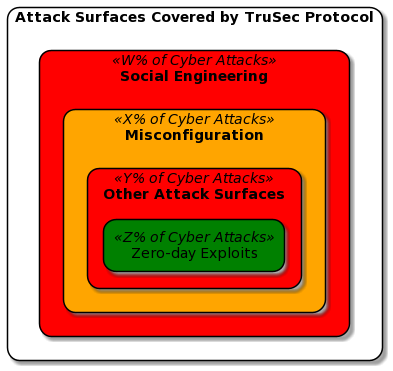
\includegraphics[width=0.50\textwidth]{images/plantuml/scope.png}
    \caption{The proposed TruSec protocol is not suited to deal with social engineering attacks, nor is it ideal for misconfiguration exploits. Instead, it is designed to increase the rate of discovery of zero day exploits.}
    \label{fig:protocol_scope}
\end{figure}
With this scope defined, one can look at how companies and ethical hackers interact with it. This is visualised in \cref{fig:interaction}.

\begin{figure}[H]
    \centering
    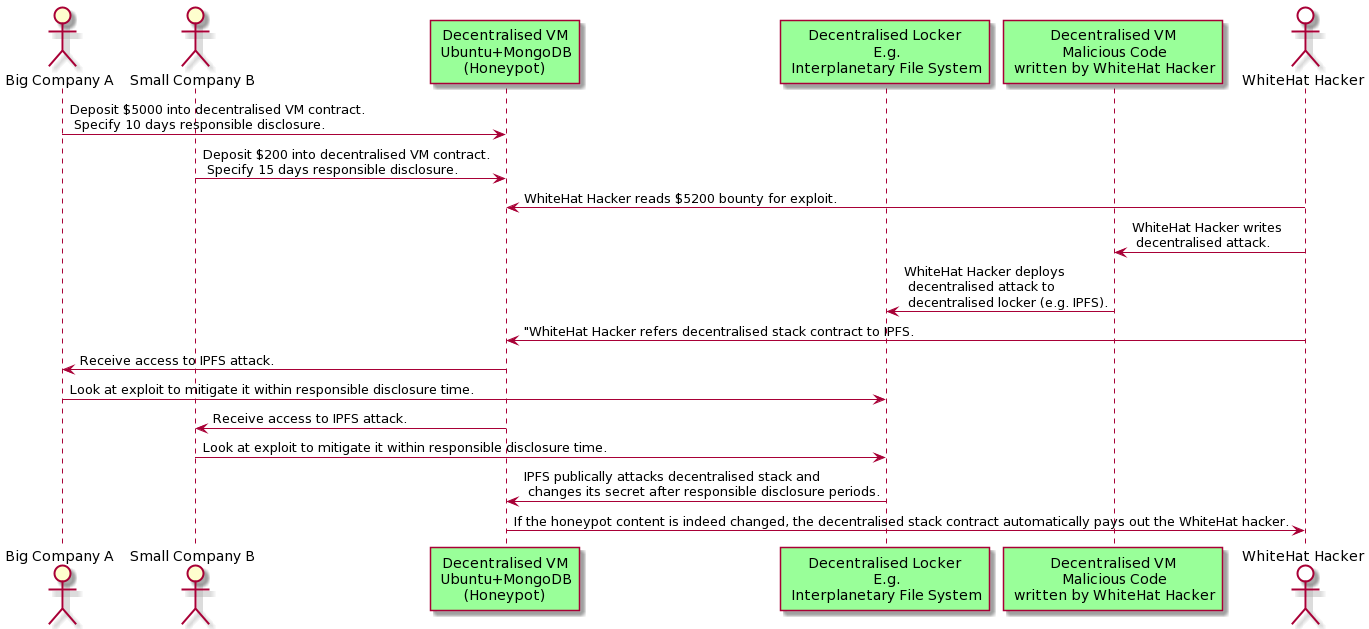
\includegraphics[width=1.0\textwidth]{images/plantuml/interaction.png}
    \caption{Rough sketch describing the interaction of the TruSec protocol. This is an ever-lasting cycle, where at the end of the process, companies can re-deploy the patched decentralised stack, and allocate new funds. Whitehat hackers can scan for new attacks.}
    \label{fig:interaction}
\end{figure}

\subsection{Development Strategy}
Based on our work on the TruCol protocol, we estimate that the development of a rough code POC would cost our student team between 3-10K euro. To have a somewhat acceptable code quality POC generated by actual employees, our first cost estimates would be in the order a few hunderd thousand euros. We imagine a fully functional and secure, audited implementation of the TruSec protocol may involve somewhere up to a million euros. 

Since we currently do not posess of the means to allocate such funds into the development of the POC, we propose the following. Our team is highly motivated to develop a detailed and thorough specification of the protocol, such that it may be presentented at Blackhat 2022 (USA). At the end of such a presentation, if accepted, we can reach out to industry to see if there is interest in developing the protocol in collaboration with some leading cyber security companies. This prevents allocating funds to a project for which no vast industry-wide interest has been generated, whilst still enabling people from all accross the world to leverage the protocol if they see fit.